\documentclass[10.5pt]{article}
\usepackage{mathpazo}
\usepackage{hyperref,url}
\usepackage[a4paper,margin=3cm]{geometry}
\usepackage{amsmath}
\usepackage{caption}
\usepackage{subcaption}
\usepackage{float}
\usepackage{graphicx}
\usepackage{cleveref}
\usepackage{listings}
\usepackage{subcaption}
\usepackage[font={small}]{caption}
\usepackage{listings}


\usepackage[backend=bibtex, sorting=none]{biblatex}
\bibliography{references}
\AtBeginBibliography{\footnotesize}

\newcommand{\Slang}{\texttt{S} }
\newcommand{\R}{\texttt{R} }
\newcommand{\Rfunction}[1]{{\texttt{#1}}}
\newcommand{\Robject}[1]{{\texttt{#1}}}
\newcommand{\Rpackage}[1]{{\mbox{\normalfont\textsf{#1}}}}
\newcommand{\E}{\mathrm{E}}
\newcommand{\Var}{\mathrm{Var}}
\newcommand{\Cov}{\mathrm{Cov}}


\usepackage{xcolor}
\definecolor{Red}{rgb}{0.7,0,0}
\definecolor{Blue}{rgb}{0,0,0.8}

\usepackage{hyperref}
\hypersetup{%
  pdfusetitle,
  bookmarks = {true},
  bookmarksnumbered = {true},
  bookmarksopen = {true},
  bookmarksopenlevel = 2,
  unicode = {true},
  breaklinks = {false},
  hyperindex = {true},
  colorlinks = {true},
  linktocpage = {true},
  plainpages = {false},
  linkcolor = {Blue},
  citecolor = {Blue},
  urlcolor = {Red},
  pdfstartview = {Fit},
  pdfpagemode = {UseOutlines},
  pdfview = {XYZ null null null}
}

%% Listings
\lstset{ 
  language=R,                     % the language of the code
  basicstyle=\footnotesize,       % the size of the fonts that are used for the code
  numbers=left,                   % where to put the line-numbers
  numberstyle=\tiny\color{gray},  % the style that is used for the line-numbers
  stepnumber=1,                   % the step between two line-numbers. If it's 1, each line will be numbered
  numbersep=5pt,                  % how far the line-numbers are from the code
  backgroundcolor=\color{white},  % choose the background color. You must add \usepackage{color}
  showspaces=false,               % show spaces adding particular underscores
  showstringspaces=false,         % underline spaces within strings
  showtabs=false,                 % show tabs within strings adding particular underscores
  rulecolor=\color{black},        % if not set, the frame-color may be changed on line-breaks within not-black text (e.g. commens (green here))
  tabsize=2,                      % sets default tabsize to 2 spaces
  captionpos=b,                   % sets the caption-position to bottom
  breaklines=true,                % sets automatic line breaking
  breakatwhitespace=false,        % sets if automatic breaks should only happen at whitespace
  title=\lstname,                 % show the filename of files included with \lstinputlisting; also try caption instead of title
  keywordstyle=\color{Blue},      % keyword style
  commentstyle=\color{orange},    % comment style
  stringstyle=\color{Red},        % string literal style
  % escapeinside={\%*}{*)},       % if you want to add a comment within your code
  % escapeinside={\%}{)},
  morekeywords={*,...}            % if you want to add more keywords to the set
} 


\newcommand{\angstrom}{\mbox{\normalfont\AA}}


\begin{document}

\title{Predicting mRNA splicing levels from sequence}
\author{CS230 Project Milestone \\[1em]
Ramya Rangan}
\date{\today}
\maketitle

%%%%%%%%%%%%%%%%%%%%%%%%%%%%%%%%%%%%%%%%%%%%%%%%%%%%%%%%
%%%%%%%%%%%%%%%%%%%%%%%%%%%%%%%%%%%%%%%%%%%%%%%%%%%%%%%%
%%%%%%%%%%%%%%%%%%%%%%%%%%%%%%%%%%%%%%%%%%%%%%%%%%%%%%%%
Code for this project is available at \texttt{https://github.com/ramyarangan/cs230\_project}.
\section{Introduction}
\subsection{Description}
The process of accurately and efficiently creating mRNA and then proteins from our genomes' DNA is critical for nearly all biological processes. Over 95\% of human genes are edited via {\bf mRNA splicing}, a process in which large sections of mRNA known as {\bf introns} are precisely recognized and removed to create the final mature mRNA that encodes the correct protein product (Figure \ref{fig:splicing}). Errors in mRNA splicing are implicated in a host of diseases from autism to cancers, with mistakes in this editing process leading to incorrect protein products and downstream disease pathways. Splicing proceeds via the recognition of specific parts of the mRNA sequence, but the patterns are complex, with mRNA sequence features influencing protein binding and RNA structures which in turn effects splicing levels. Though it is of great interest to understand the rules that govern the extent to which splicing occurs at a particular position in mRNA, we do not yet have predictive models that can determine splicing efficiency from an mRNA's sequence. Here we explore CNN and RNN approaches for predicting splicing efficiency values given an RNA sequence context.
\begin{figure}[H]
\centering
\begin{subfigure}{.4 \textwidth}
\centering
\caption{} 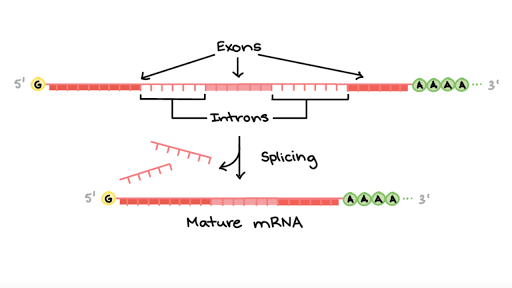
\includegraphics[width=6cm]{splicing_graphic.png} 
\label{fig:splicing}
\end{subfigure}
\begin{subfigure}{.5 \textwidth}
\centering
\caption{}  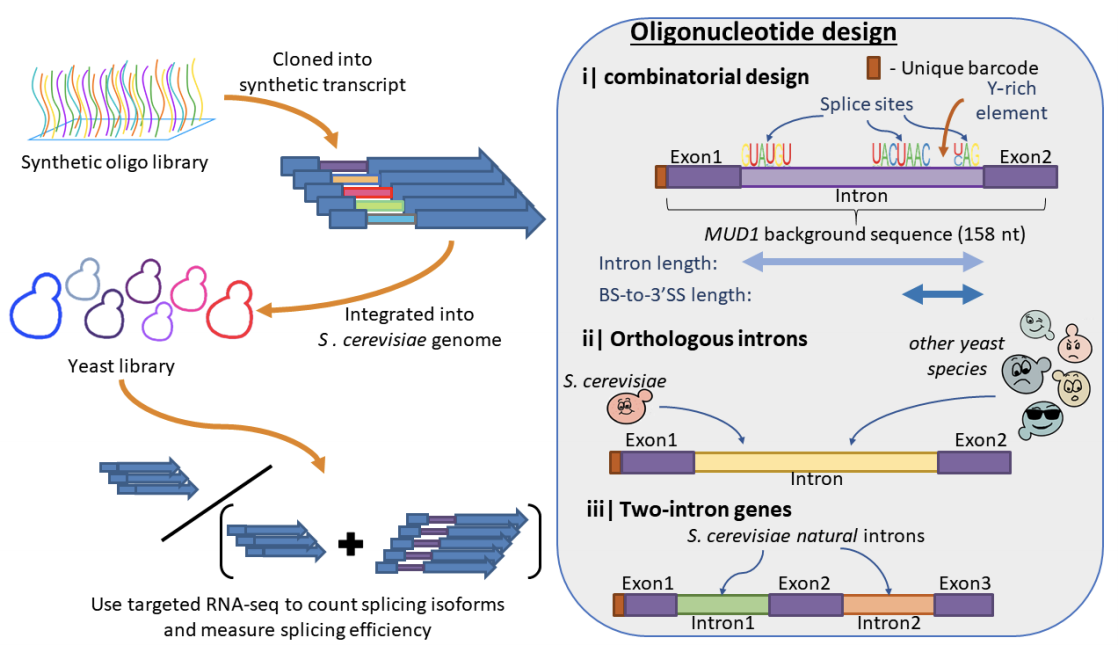
\includegraphics[width=6cm]{dataset_overview_pilpel.png} 
\label{fig:dataset}
\end{subfigure}
\caption{a) mRNA splicing overview. b) Schematic depicting the library of splicing efficiency measurements. Data and figure from Schirman, et al. bioRxiv 2021 [1].}
\end{figure}
\subsection{Prior work}
Large datasets have become available over the last decade that can aid in developing models predicting splicing efficiency from mRNA sequence. In some cases, splicing efficiency readouts have been obtained for designed libraries of thousands to millions of constructs ([1], [2]), and simple algorithms have achieved moderate predictive power for splicing efficiency (in the case of [1], gradient boosting models with a small set of features achieves 0.77 Pearson correlation and in [2], a regression model explains 55-75\% of variation in splicing levels). Large collections of naturally occurring mRNA's have also been assayed, providing another opportunity for learning models to predict splicing efficiency. In SpanR, neural networks were trained based on feature sets with over 1000 hand-designed features, yielding an $R^2$ value of 0.65 between predicted and true splicing efficiency values [3]. Deep learning approaches have already shown promise, with a 32-layer CNN SpliceAI successfully predicting a binary splicing or not splicing outcome given a position of interest and a large 10,000 sequence context [4]. However, deep learning approaches have not yet been used to predict continuous splicing efficiency values given an mRNA sequence, a prediction task critical for understanding downstream consequences of disease sequence variants.
\subsection{Contribution}
Here, we explore the ability of deep learning to predict the extent to which splicing happens at a particular position (value from 0 to 1) given a complete mRNA sequence including both the intron and surrounding sequence, training models using a recently collected dataset of splicing efficiency values for tens of thousands of constructs in {\it Saccharomyces cerevisiae} (yeast). We compare a baseline model that uses simple sequence heuristics with a CNN and RNN network architecture, finding [FILL IN].
\section{Dataset}
\subsection{Data composition}
We use the dataset collected by Shirman, et al. [1] of splicing efficiency values for a library of 14888 designed sequence variants in yeast (Figure \ref{fig:dataset}). Each datapoint consists of a sequence of length 1615 nucleotides (A, C, T, or G) along with a corresponding splicing efficiency value (real values from 0 to 1), measured through RNA sequencing. The dataset consists of five library types with different synthetic sequence design strategies to probe different backgrounds (12376 sequences) and two library types based on naturally occurring intron variants in {\it S. cerevisiae} and other related yeast species (2501 sequences). 
\newline \\
To split the dataset into training, dev, and testing data, we used 90\% of each library type in the training set, and 5\% of each library type in the dev and test sets. By sampling these splits within library types, we ensured that the dev and test set have the same distribution, and we made sure that near-identical sequences were not shared between the training, dev, and test sets. We can augment the training dataset with additional negative examples by using intervals from the yeast genome that do not overlap with naturally occurring spliced mRNA's, assigning these examples to the splicing efficiency value of 0. 
\subsection{Evaluation metrics}
Since we are predicting a real-valued outcome, we use a mean-squared error regression loss function as implemented in Keras, and we will use a ReLU activation function for the final node in the neural network models. We tune models by evaluating them on the dev dataset, and we evaluate final models on the test dataset.
\section{Methods}
\subsection{Baseline Model}
We first tested a baseline model using simple sequence heuristics to assign sequences to a splicing efficiency value. For each sequence in the dev set, we predicted its splicing efficiency value by comparing similarity to wildtype yeast mRNA that have introns that are spliced. If the sequence is not similar to known spliced mRNA's in yeast, we predict a splicing efficiency of 0, and if it is similar, we assign the predicted splicing efficiency value to be  the average splicing efficiency value from the training set (computed using only sequences with splicing level above $\epsilon = 0.001$). \newline \\
To evaluate similarity of sequences in the dev set to wildtype yeast spliced mRNA's we used the following heuristics. At a first approximation, splicing occurs when the cell's splicing machinery recognizes three short key sequences in mRNAs: the {\bf 5' splice site} (6 nucleotides at the start of an intron), {\bf branch site} (8 nucleotides in the latter portion of the intron), and {\bf 3' splice site} (3 nucleotides at the end of the intron). First we compute the position weight matrix (nucleotide distribution) for sequence motifs at each of these three key sequences using wildtype yeast mRNAs. We additionally compute two length distributions from wildtype introns: the full length of the intron, and the length between the branch site and 3' splice site. For a tested sequence to be marked as similar to wildtype yeast splicing mRNA's, we require that sequences' score against the position weight matrix and length distributions fall within the 95th percentile of wildtype introns. \newline \\
When the Baseline Model is used to predict splicing efficiency values for the development set, the mean-squared error loss on the dev set is {\bf 0.0638}, compared to the mean-squared error loss of {\bf 0.308} for a random model that predicts uniform random values from 0 to 1 for all dev set examples.
\subsection{CNN Model}
CNN models have been used fruitfully to predict binary splicing outcomes from mRNA sequence [4]. We will implement and train a CNN model with convolution layers, pooling layers, and fully connected layers to predict splicing efficiency values.
\subsection{RNN Model}
RNN models have been shown to capture long-range base-pairing interactions in RNA sequences [5], which have been shown to play a role in regulating mRNA splicing efficiency. These long-range interactions represent second-order effects that would not be captured by the Baseline Model. We will implement and train an RNN, and evaluate its performance on the development set.
\section{Results}
\section{Discussion and Conclusion}

\begin{thebibliography}{9}
\bibitem{pilpel} 
Schirman, D., Yakhini, Z., Dahan, O., Pilpel, Y.
\textit{Sequence determinants and evolution of constitutive and alternative splicing in yeast species}. 2021. bioRxiv. 

\bibitem{seelig} 
Rosenberg, A.B., Patwardhan, R.P., Shendure, J., Seelig, G.
\textit{Learning the sequence determinants of alternative splicing from millions of random sequences.}. 2015. Cell, 163 (698-711). 

\bibitem{spanr}
Xiong, H.Y., Alipanahi, B., Lee, L.J., et al. 
\textit{The human splicing code reveals new insights into the genetic determinants of disease.} 2015. Science, 347 (1254806).

\bibitem{spliceai} 
Jaganathan, K., Panagiotopoulou, S. K., McRae, J.F., et al. 
\textit{Predicting splicing from primary Sequence with deep learning}. 2019. Cell, 176 (535-548). 

\bibitem{rnn} 
Wu, M., Andreasson, J.O.L, Kladwang, W., et al. \textit{Prospects for recurrent neural network models to learn RNA
biophysics from high-throughput data}. 2018. bioRxiv.
\end{thebibliography}


\end{document}
\subsection*{(a)}


\end{document}